\documentclass[12pt,a4paper]{article}

% -------------------------------------------------------
% Pacotes
% -------------------------------------------------------
\usepackage[utf8]{inputenc}
\usepackage[T1]{fontenc}
\usepackage[brazilian]{babel}
\usepackage{amsmath,amssymb}
\usepackage{graphicx}
\usepackage{float}
\usepackage{array}
\usepackage{booktabs}
\usepackage{longtable}
\usepackage{geometry}
\usepackage{setspace}
\usepackage{indentfirst}
\usepackage{caption}
\usepackage[table]{xcolor}
\usepackage[most]{tcolorbox}
\usepackage{hyperref}

% -------------------------------------------------------
% Configurações gerais
% -------------------------------------------------------
\geometry{
left=3cm,
right=2cm,
top=3cm,
bottom=2cm
}

\onehalfspacing
\setlength{\parindent}{1.25cm}
\setlength{\parskip}{0.15cm}
\setcounter{tocdepth}{2}
\setcounter{secnumdepth}{3}

\hypersetup{
colorlinks=true,
linkcolor=black,
urlcolor=black,
citecolor=black
}

% -------------------------------------------------------
% Caixa para cálculos
% -------------------------------------------------------
\newtcolorbox{caixacalculo}[1]{
enhanced,
breakable,
colback=gray!6,
colframe=black!65,
title=\textbf{#1},
fonttitle=\normalsize,
coltitle=black,
attach boxed title to top left={xshift=0.4cm,yshift=-2mm},
boxed title style={colback=gray!20,colframe=black!65},
arc=2mm,
boxrule=0.6pt,
left=4mm,
right=4mm,
top=4mm,
bottom=4mm
}

% -------------------------------------------------------
% Informações do relatório
% -------------------------------------------------------
\newcommand{\instituicao}{Instituto Federal de Educação, Ciência e Tecnologia de Mato Grosso}
\newcommand{\campus}{Campus Pontes e Lacerda -- Fronteira Oeste}
\newcommand{\curso}{Bacharelado em Engenharia Elétrica}
\newcommand{\disciplina}{Circuitos Elétricos II}
\newcommand{\professor}{Professor da disciplina}
\newcommand{\titulo}{Relatório Acadêmico -- Experimento 5}
\newcommand{\subtitulo}{Medição da potência elétrica em motor de indução trifásico tipo gaiola de esquilo, 2 polos, 24 V em ligação delta}

\begin{document}
\hypersetup{pageanchor=false}
\pagenumbering{gobble}

% -------------------------------------------------------
% Capa
% -------------------------------------------------------
\begin{titlepage}
\thispagestyle{empty}

\begin{center}

\IfFileExists{logo-ifmt.png}{

\includegraphics[width=8cm]{logo-ifmt.png}
}{
\fbox{
\begin{minipage}[c][3cm][c]{5cm}
\centering
Espaço reservado para o logo do IFMT
\end{minipage}
}
}

\vspace{1cm}

{\large \textbf{\instituicao}}\\
\vspace{0.2cm}
{\large \textbf{\campus}}\\
\vspace{0.2cm}
{\large \curso}

\vspace{1.6cm}
\vspace{2.2cm}

{\large Nicoly Canteiro Araújo e colegas de grupo}

\vspace{4.4cm}
\vspace{0.8cm}

\begin{minipage}{0.9\textwidth}
\centering
{\large \textbf{\subtitulo}}
\end{minipage}

\vfill

{\large Pontes e Lacerda -- MT}\\
{\large 2026}

\end{center}
\end{titlepage}

% -------------------------------------------------------
% Folha de rosto / Sobrecapa
% -------------------------------------------------------
\begin{titlepage}
\thispagestyle{empty}

\begin{center}

\IfFileExists{logo-ifmt.png}{

\includegraphics[width=8.0cm]{logo-ifmt.png}
}{
\fbox{
\begin{minipage}[c][2.8cm][c]{5cm}
\centering
Espaço reservado para o logo do IFMT
\end{minipage}
}
}

\vspace{4cm}
\vspace{0.8cm}

\begin{minipage}{0.9\textwidth}
\centering
{\large \textbf{\subtitulo}}
\end{minipage}

\end{center}

\vspace{3cm}

\begin{flushright}
\begin{minipage}{8.5cm}
Relatório acadêmico sobre a medição de potência elétrica em um motor de indução trifásico tipo gaiola de esquilo, com 2 polos e tensão de 24 V em ligação delta.

O trabalho foi desenvolvido na disciplina de Circuitos Elétricos II, do curso de Bacharelado em Engenharia Elétrica do Instituto Federal de Educação, Ciência e Tecnologia de Mato Grosso, Campus Pontes e Lacerda -- Fronteira Oeste.

\vspace{1.5cm}

\textbf{Professor:} \professor
\end{minipage}
\end{flushright}

\vfill

\begin{center}
Pontes e Lacerda -- MT\\
2026
\end{center}

\end{titlepage}

% -------------------------------------------------------
% Sumário
% -------------------------------------------------------
\clearpage
\hypersetup{pageanchor=true}
\pagenumbering{arabic}
\tableofcontents
\newpage

% -------------------------------------------------------
\section{Resumo}
% -------------------------------------------------------

Este relatório apresenta o ensaio de um motor de indução trifásico tipo gaiola de esquilo, com 2 polos e tensão de 24 V em ligação delta. A prática teve como objetivo observar o funcionamento do motor com diferentes cargas e analisar as principais grandezas medidas em laboratório.

Durante o experimento, foram registrados valores de tensão, corrente, potência, velocidade e posição do braço do freio eletromagnético. Com esses dados, foram calculados a potência absorvida, a potência de saída, o torque, o fator de potência e o rendimento.

De forma geral, o experimento ajudou a entender como o motor se comporta durante a aplicação de carga. Alguns resultados ficaram fora do esperado, principalmente os rendimentos acima de 100\%, indicando possíveis erros de medição, ajustes do equipamento ou variações durante o ensaio.

\newpage

% -------------------------------------------------------
\section{Introdução}
% -------------------------------------------------------

Os motores de indução trifásicos são muito utilizados em sistemas elétricos e industriais por serem resistentes, simples de operar e eficientes em várias aplicações. O motor tipo gaiola de esquilo é um dos modelos mais comuns, pois possui construção prática e boa durabilidade.

Seu funcionamento ocorre pela ação do campo magnético girante produzido no estator. Esse campo induz corrente no rotor e gera o torque responsável pelo movimento do eixo. Por isso, grandezas como corrente, potência, velocidade, torque, fator de potência e rendimento são importantes para avaliar o desempenho do motor.

Neste experimento, a potência elétrica foi medida pelo método dos dois wattímetros. Esse método permite determinar a potência ativa total em um sistema trifásico por meio da soma algébrica das leituras dos instrumentos.

\newpage

% -------------------------------------------------------
\section{Objetivo}
% -------------------------------------------------------

O objetivo deste experimento foi analisar o comportamento de um motor de indução trifásico tipo gaiola de esquilo, quando submetido a diferentes níveis de carga mecânica.

Também foram observados os seguintes pontos:

\begin{itemize}
\item realizar a ligação do motor em delta;
\item conectar o motor à alimentação trifásica;
\item medir tensão, corrente, potência e velocidade;
\item aplicar o método dos dois wattímetros;
\item calcular potência absorvida, potência de saída, torque, fator de potência e rendimento;
\item comparar os resultados obtidos com o comportamento esperado para esse tipo de motor.
\end{itemize}

\newpage

% -------------------------------------------------------
\section{Material Utilizado}
% -------------------------------------------------------

Para a realização do experimento, foram utilizados os seguintes materiais e equipamentos:

\begin{itemize}
\item 1 estator de máquina CA e rotor tipo gaiola de esquilo;
\item 1 módulo de alimentação \textbf{DL 10281};
\item 1 módulo de medição \textbf{DL 10282N};
\item 1 suporte adaptador \textbf{DL 10284};
\item 1 freio eletromagnético \textbf{DL 10300A} com braços;
\item 1 multímetro digital \textbf{MY60};
\item 1 tacômetro digital \textbf{DL 2026}.
\end{itemize}

% -------------------------------------------------------
\section{Procedimento Experimental}
% -------------------------------------------------------

\subsection{Montagem do conjunto}

Primeiro, foi montado o conjunto formado pelo motor de indução trifásico e pelo freio eletromagnético. Em seguida, foram feitas as ligações elétricas conforme o esquema indicado para a prática.

O motor foi ligado em delta e os instrumentos foram posicionados para medir tensão, corrente, potência elétrica e velocidade de rotação durante o ensaio.

\subsection{Medições}

A carga mecânica foi aplicada aos poucos, alterando a posição do peso no braço do freio eletromagnético. Para cada ponto de operação, foram anotados os valores medidos no experimento.

Depois das medições, os dados foram usados para calcular as principais grandezas do motor, como potência absorvida, potência de saída, torque, fator de potência e rendimento.

\subsection{Dados obtidos e cálculos realizados}

As fórmulas utilizadas foram organizadas em caixas para deixar os cálculos separados da explicação. Isso facilita a leitura e deixa o relatório mais claro.

\begin{caixacalculo}{Potência elétrica absorvida pelo motor}
A potência absorvida foi calculada pela soma das leituras dos dois wattímetros:
\begin{equation*}
P_{in}=P_{13}+P_{23}
\end{equation*}

Nessa fórmula, $P_{in}$ é a potência elétrica total absorvida pelo motor. Os valores $P_{13}$ e $P_{23}$ são as leituras dos wattímetros.
\end{caixacalculo}

\begin{caixacalculo}{Torque mecânico}
O torque foi calculado multiplicando o peso aplicado pelo braço de alavanca:
\begin{equation*}
M=G\cdot b
\end{equation*}

Em que $M$ é o torque, $G$ é o peso aplicado e $b$ é a distância do braço de alavanca.
\end{caixacalculo}

\begin{caixacalculo}{Potência mecânica de saída}
A potência de saída foi calculada usando a velocidade de rotação e o torque:
\begin{equation*}
P_{out}=0{,}1047\cdot n\cdot M
\end{equation*}

Nessa expressão, $P_{out}$ é a potência mecânica no eixo, $n$ é a velocidade de rotação e $M$ é o torque.
\end{caixacalculo}

\begin{caixacalculo}{Fator de potência}
O fator de potência foi calculado pela relação entre a potência ativa e a potência aparente do sistema trifásico:
\begin{equation*}
\cos\varphi=\frac{P_{in}}{\sqrt{3}\cdot U\cdot I}
\end{equation*}

Esse valor mostra se a energia fornecida ao motor está sendo bem aproveitada na forma de potência ativa.
\end{caixacalculo}

\begin{caixacalculo}{Rendimento do motor}
O rendimento foi calculado comparando a potência de saída com a potência absorvida:
\begin{equation*}
\eta=\frac{P_{out}}{P_{in}}\cdot100
\end{equation*}

O resultado é dado em porcentagem e indica o quanto da energia recebida foi transformada em potência útil no eixo.
\end{caixacalculo}

% -------------------------------------------------------
\subsection{Tabela de dados e resultados calculados}
% -------------------------------------------------------

\begin{table}[H]
\centering
\caption{Dados experimentais e resultados calculados}
\vspace{0.2cm}

\renewcommand{\arraystretch}{1.2}
\setlength{\tabcolsep}{2pt}
\scriptsize
\begin{tabular}{|c|c|c|c|c|c|c|c|c|c|c|c|}
\hline
\textbf{U} & \textbf{I} & \textbf{$P_{13}$} & \textbf{$P_{23}$} & \textbf{$P_{in}$} & \textbf{$\cos\varphi$} & \textbf{G} & \textbf{b} & \textbf{M} & \textbf{n} & \textbf{$P_{out}$} & \textbf{$\eta$} \\
\textbf{(V)} & \textbf{(A)} & \textbf{(W)} & \textbf{(W)} & \textbf{(W)} &  & \textbf{(N)} & \textbf{(m)} & \textbf{(Nm)} & \textbf{(min$^{-1}$)} & \textbf{(W)} & \textbf{(\%)} \\
\hline
25,40 & 4,151 & 106 & 55,05 & 161,05 & 0,882 & 3,5 & 0 & 0 & 3412 & 0 & 0 \\
\hline
25,83 & 3,040 & 77,98 & 34,43 & 112,41 & 0,827 & 3,5 & 0,025 & 0,0875 & 3500 & 32,06 & 28,52 \\
\hline
25,96 & 2,756 & 71,06 & 28,11 & 99,17 & 0,800 & 3,5 & 0,05 & 0,175 & 3525 & 64,59 & 65,13 \\
\hline
25,31 & 2,49 & 63,01 & 21,38 & 84,39 & 0,773 & 3,5 & \cellcolor{red!85}0,075 & 0,2625 & 3548 & 97,51 & \cellcolor{red!85}115,55 \\
\hline
25,98 & 2,29 & 57,41 & 17,71 & 75,12 & 0,729 & 3,5 & \cellcolor{red!85}0,1 & 0,35 & 3562 & 130,53 & \cellcolor{red!85}173,76 \\
\hline
26,11 & 1,815 & 41,06 & 1,464 & 42,524 & 0,518 & 3,5 & \cellcolor{red!85}0,125 & 0,4373 & 3604 & 165,01 & \cellcolor{red!85}388,04 \\
\hline
26,17 & 1,757 & 37,58 & -3,17 & 34,41 & 0,432 & 3,5 & \cellcolor{red!85}0,15 & 0,525 & 3614 & 198,65 & \cellcolor{red!85}577,31 \\
\hline
\end{tabular}

\end{table}

\vspace{0.3cm}

\noindent\textbf{Observação:} Os rendimentos acima de 100\% não são fisicamente possíveis, pois o motor não pode entregar mais potência do que recebe. Esses valores indicam possíveis erros de leitura, variação nos instrumentos, ajuste do freio ou alguma inconsistência nos dados coletados. Mesmo assim, a tabela ajuda a observar o comportamento geral do motor durante o ensaio.

% -------------------------------------------------------
\subsection[Diagrama de desempenho do motor]{Diagrama da corrente absorvida $I$, do fator de potência $\cos\varphi$, da velocidade $n$ e do rendimento $\eta$ em função da potência de saída $P_{out}$.}
% -------------------------------------------------------

\vspace{0.4cm}

\begin{figure}[H]
\centering

\IfFileExists{grafico-motor.png}{
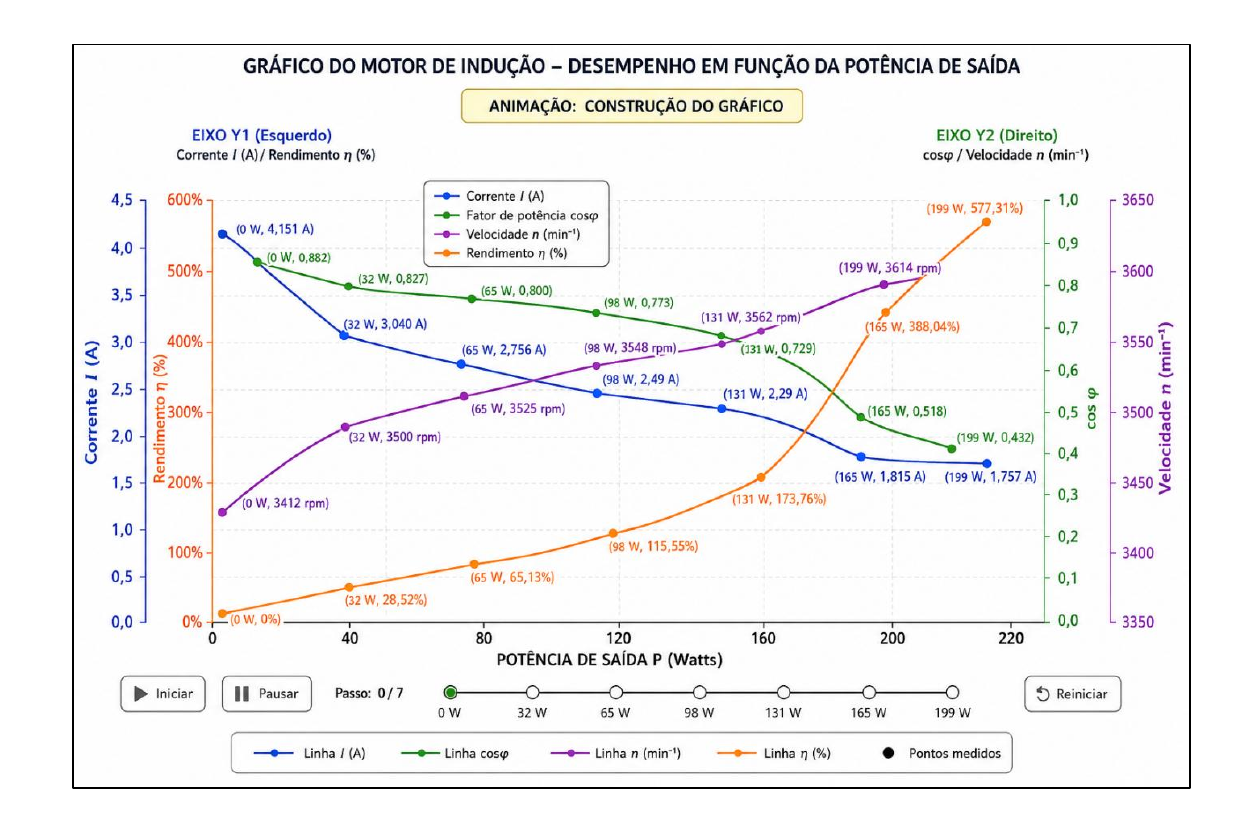
\includegraphics[width=0.88\textwidth]{grafico-motor.png}
}{
\fbox{
\begin{minipage}[c][8cm][c]{0.88\textwidth}
\centering
\textbf{Espaço reservado para o gráfico do motor de indução}\\[0.4cm]
Inserir aqui a imagem do diagrama contendo a corrente absorvida $I$, o fator de potência $\cos\varphi$, a velocidade $n$ e o rendimento $\eta$ em função da potência de saída $P_{out}$.
\end{minipage}
}
}

\caption{Desempenho do motor de indução em função da potência de saída}
\label{fig:grafico-motor}
\end{figure}

% -------------------------------------------------------
\subsection{Registros fotográficos do experimento}
% -------------------------------------------------------

As imagens desta seção mostram registros feitos durante a prática em laboratório. Elas ajudam a documentar a montagem, os equipamentos utilizados e alguns momentos do ensaio.

Essas fotografias não fazem parte dos cálculos. Elas servem apenas como apoio visual para mostrar como o experimento foi realizado.

\begin{figure}[H]
\centering

\IfFileExists{foto-simulacao-01.png}{
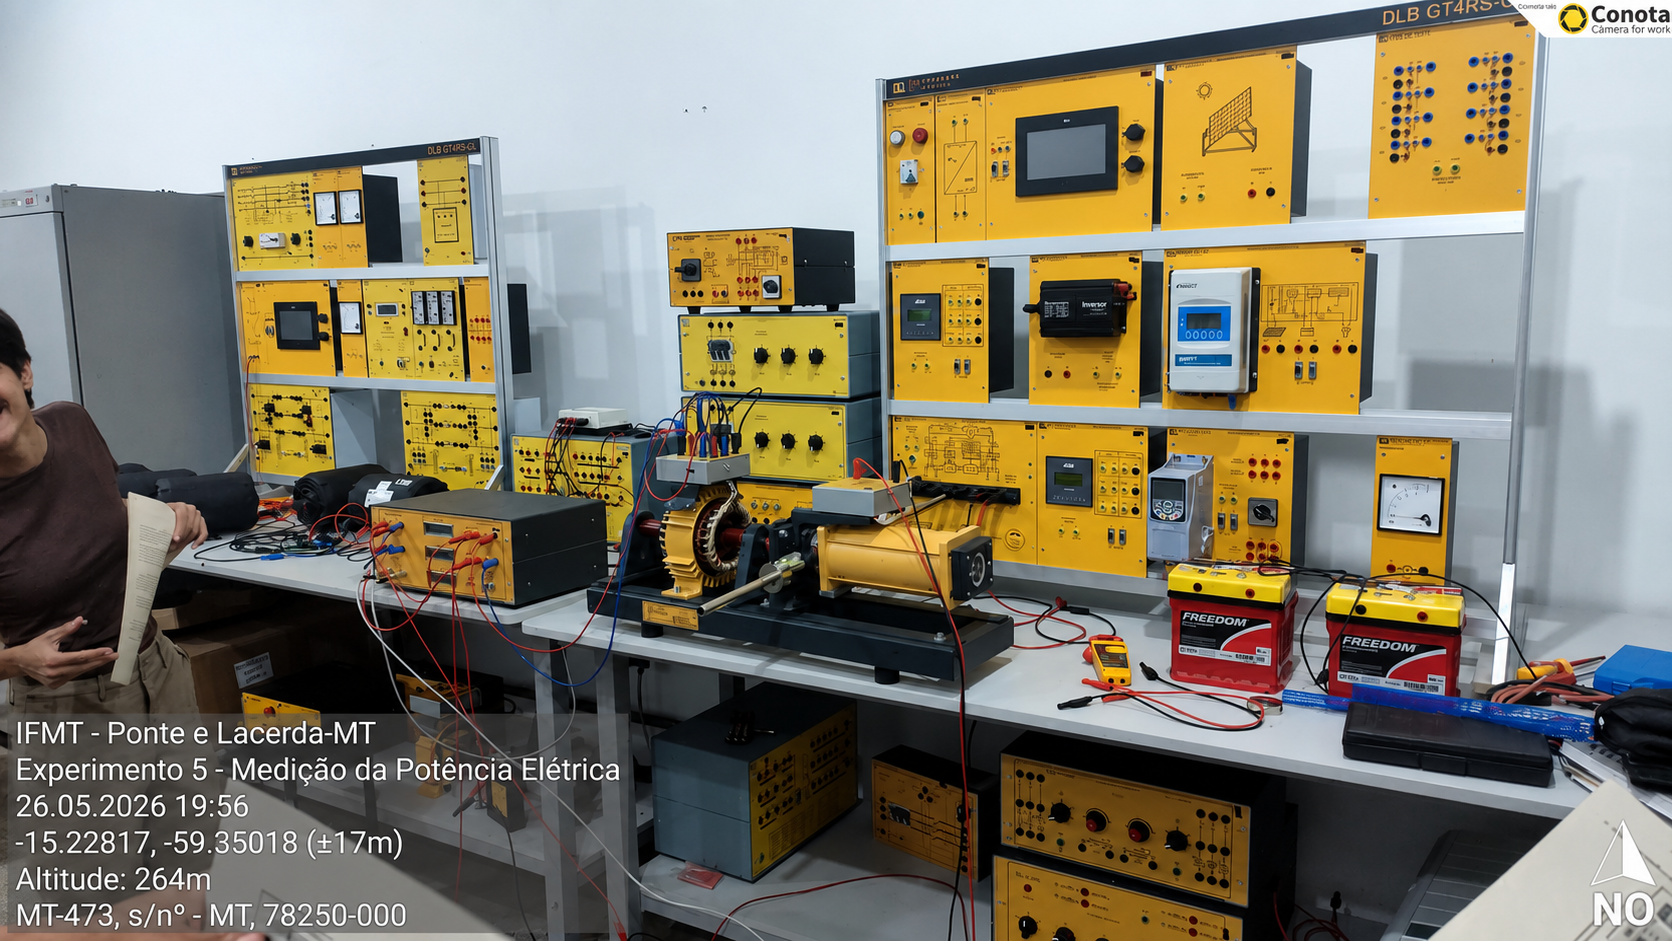
\includegraphics[width=0.88\textwidth]{foto-simulacao-01.png}
}{
\fbox{
\begin{minipage}[c][7cm][c]{0.88\textwidth}
\centering
\textbf{Espaço reservado para registro fotográfico do laboratório}\\[0.3cm]
Inserir aqui a fotografia feita durante os testes físicos no laboratório.
\end{minipage}
}
}

\caption{Registro fotográfico da montagem realizada antes dos testes do motor}
\label{fig:foto-simulacao-01}
\end{figure}

\vspace{0.3cm}

\begin{figure}[H]
\centering

\IfFileExists{foto-simulacao-02.png}{
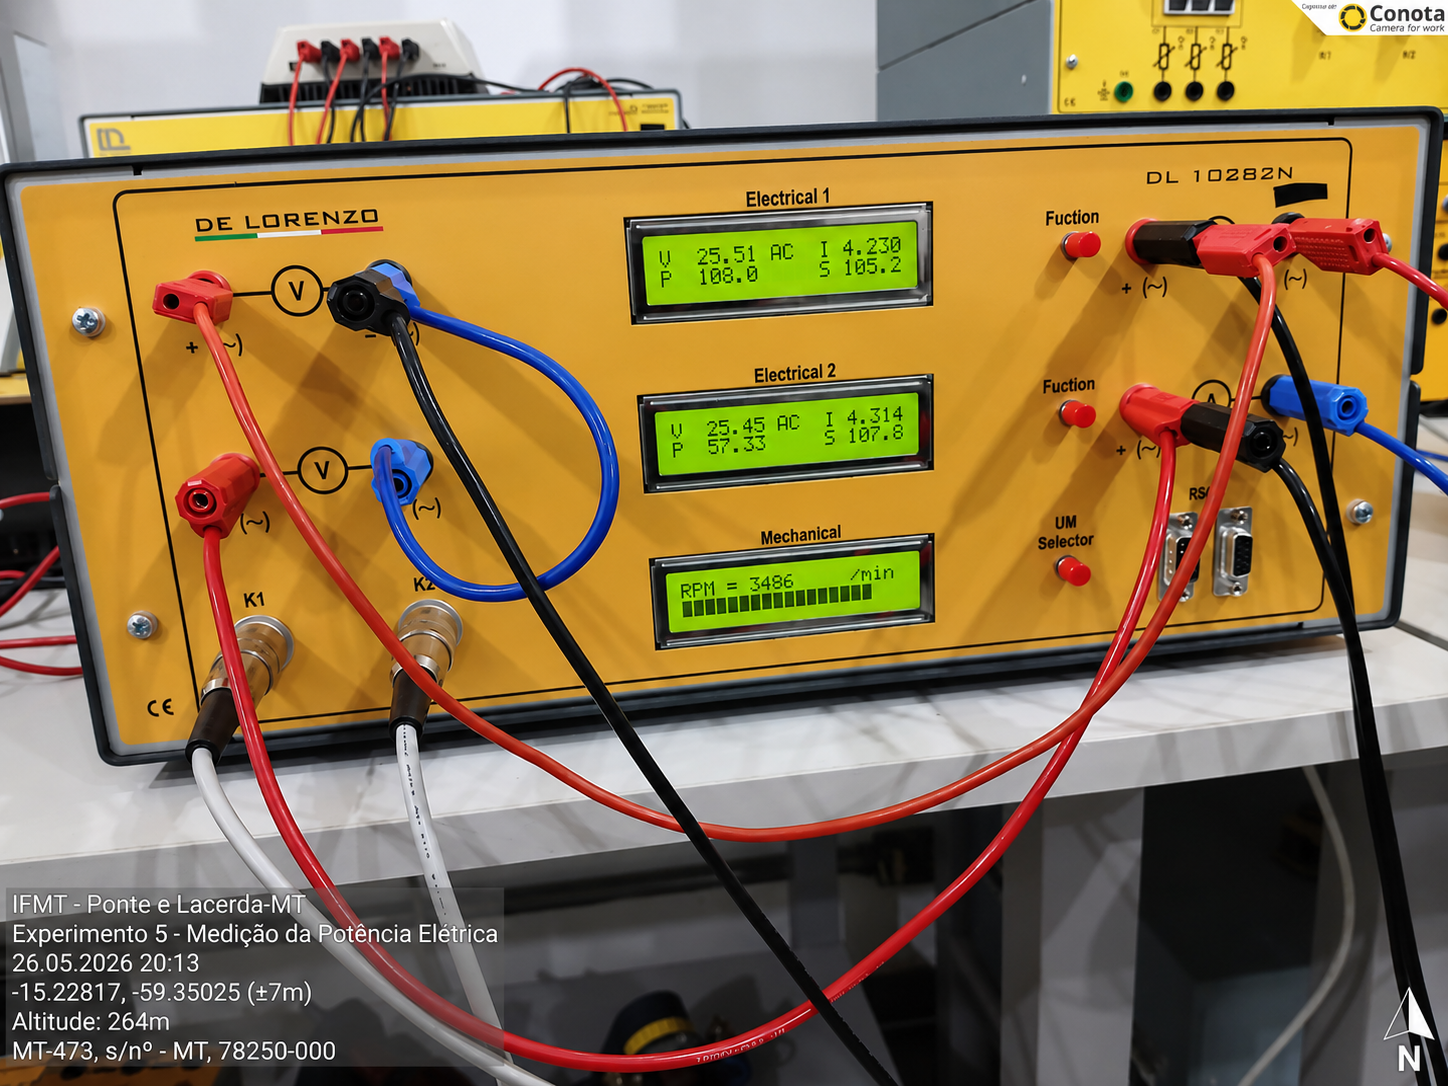
\includegraphics[width=0.88\textwidth]{foto-simulacao-02.png}
}{
\fbox{
\begin{minipage}[c][7cm][c]{0.88\textwidth}
\centering
\textbf{Espaço reservado para registro fotográfico do laboratório}\\[0.3cm]
Inserir aqui a fotografia complementar feita durante os testes físicos no laboratório.
\end{minipage}
}
}

\caption{Registro fotográfico dos testes físicos realizados em laboratório}
\label{fig:foto-simulacao-02}
\end{figure}

\vspace{0.3cm}

\begin{figure}[H]
\centering

\IfFileExists{foto-simulacao-04.png}{
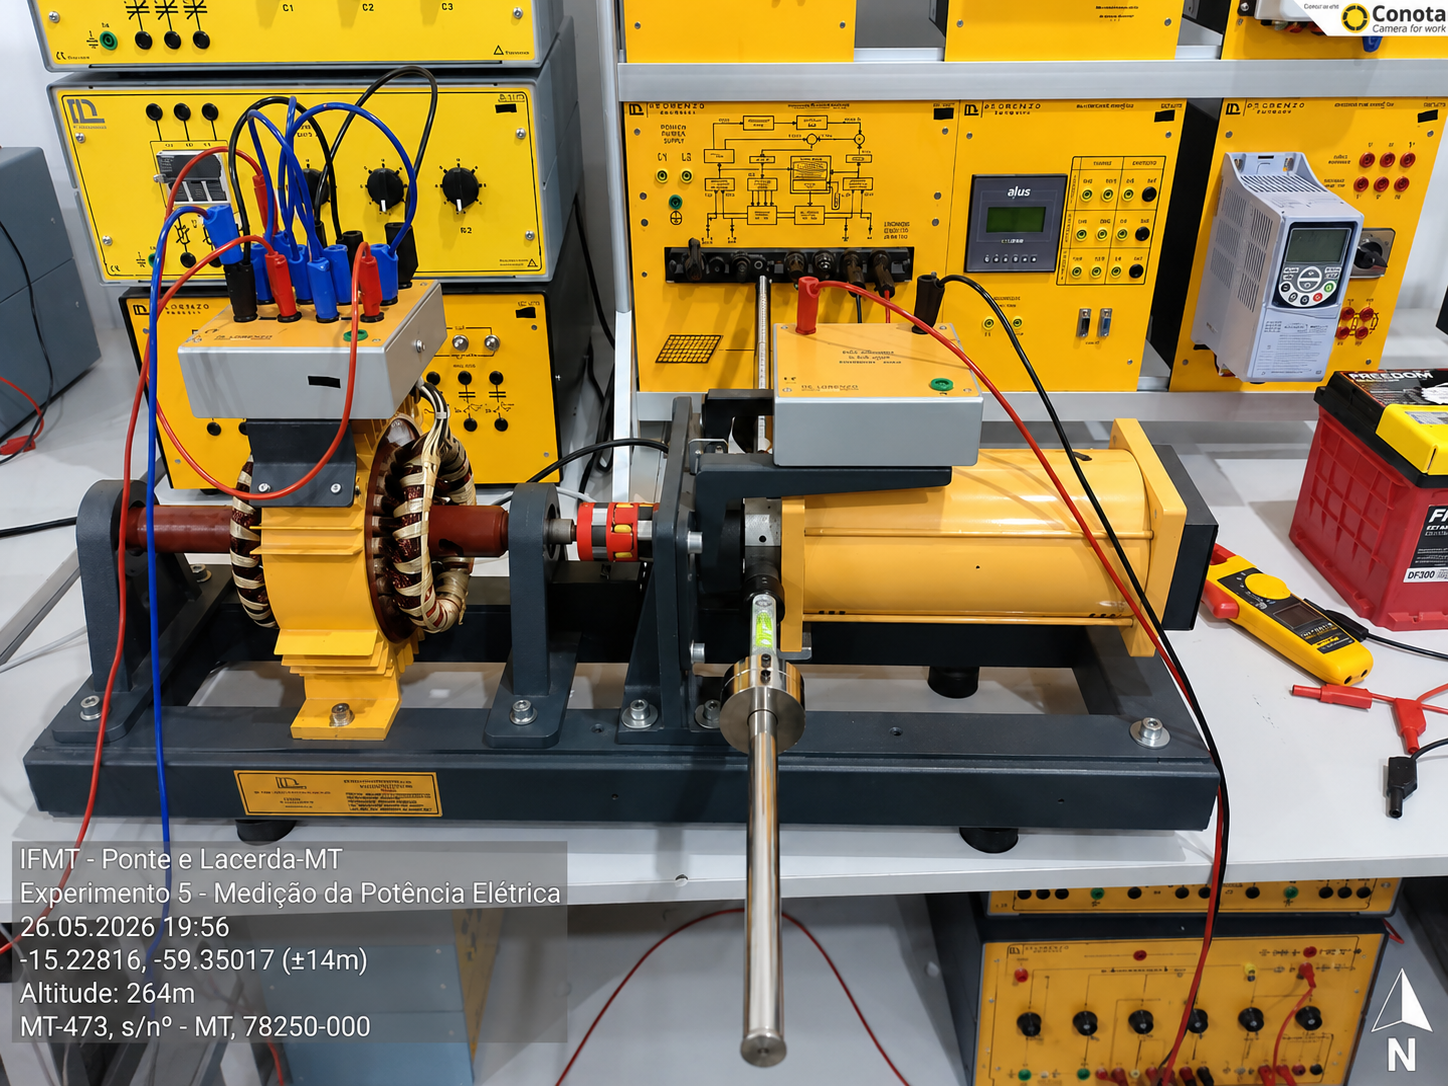
\includegraphics[width=0.88\textwidth]{foto-simulacao-04.png}
}{
\fbox{
\begin{minipage}[c][7cm][c]{0.88\textwidth}
\centering
\textbf{Espaço reservado para registro fotográfico da montagem}\\[0.3cm]
Inserir aqui a fotografia 4, referente à montagem experimental.
\end{minipage}
}
}

\caption{Registro fotográfico da montagem experimental realizada em laboratório}
\label{fig:foto-simulacao-04}
\end{figure}

\vspace{0.3cm}

\begin{figure}[H]
\centering

\IfFileExists{foto-simulacao-05.png}{
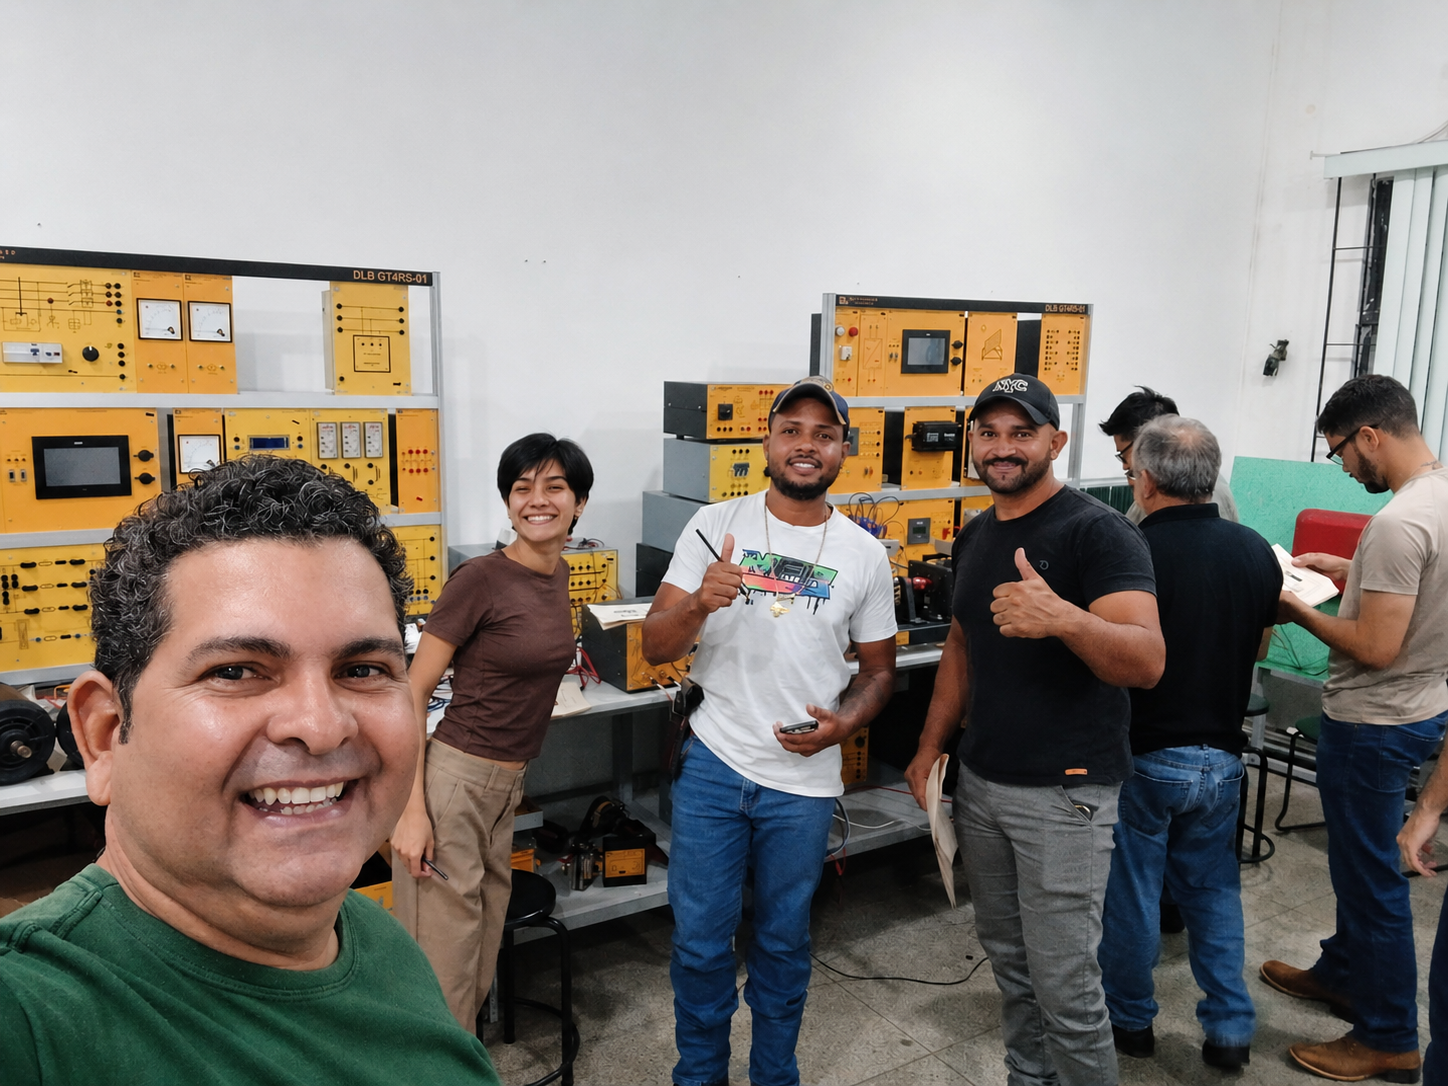
\includegraphics[width=0.88\textwidth]{foto-simulacao-05.png}
}{
\fbox{
\begin{minipage}[c][7cm][c]{0.88\textwidth}
\centering
\textbf{Espaço reservado para registro fotográfico em equipe}\\[0.3cm]
Inserir aqui a fotografia 5, referente ao registro da equipe durante a prática.
\end{minipage}
}
}

\caption{Registro fotográfico da equipe durante a realização do experimento}
\label{fig:foto-simulacao-05}
\end{figure}

% -------------------------------------------------------
\section{Resposta às perguntas propostas}
% -------------------------------------------------------

\subsection{Princípio de funcionamento do método dos dois wattímetros}

O método dos dois wattímetros é usado para medir a potência ativa total em sistemas trifásicos. Nele, dois wattímetros são ligados em duas fases do circuito, usando a terceira fase como referência para as bobinas de tensão.

\begin{caixacalculo}{Potência total pelo método dos dois wattímetros}
A potência ativa total é calculada pela soma algébrica das duas leituras:
\begin{equation*}
P_{total}=P_1+P_2
\end{equation*}

Quando uma leitura aparece negativa, ela deve continuar com sinal negativo na soma. Isso pode acontecer quando o fator de potência está baixo.
\end{caixacalculo}

Esse método facilita a medição da potência total do sistema trifásico, sem precisar medir cada fase separadamente.

\subsection{Variação da corrente absorvida com o aumento da carga}

Em um motor de indução, o esperado é que a corrente aumente quando a carga mecânica também aumenta. Isso ocorre porque o motor precisa de mais energia elétrica para produzir maior torque no eixo.

\begin{caixacalculo}{Relação entre potência, tensão, corrente e fator de potência}
A potência em um sistema trifásico pode ser representada por:
\begin{equation*}
P=\sqrt{3}\cdot U\cdot I\cdot \cos\varphi
\end{equation*}

Assim, quando a carga aumenta, a corrente tende a subir para atender à maior necessidade de potência.
\end{caixacalculo}

Nos dados obtidos, a corrente diminuiu conforme a carga aumentou. Esse comportamento não é o mais esperado e pode estar ligado a erro de leitura, variação na alimentação, ajuste do freio ou limitação dos equipamentos.

\subsection{Relação entre potência de saída e rendimento}

O rendimento mostra quanto da potência elétrica recebida pelo motor foi convertida em potência mecânica útil. Em um motor real, esse valor deve ser menor que 100\%, pois sempre existem perdas no processo.

\begin{caixacalculo}{Cálculo do rendimento}
O rendimento é calculado por:
\begin{equation*}
\eta=\frac{P_{out}}{P_{in}}\cdot100
\end{equation*}

Quando o resultado passa de 100\%, significa que existe alguma inconsistência nas medições ou nos dados usados.
\end{caixacalculo}

No experimento, alguns pontos apresentaram rendimento acima de 100\%. Isso não representa o comportamento real do motor, mas indica que houve alguma limitação ou erro durante a coleta dos dados.

\subsection{Por que a velocidade diminui levemente com o aumento da carga?}

Em motores de indução, a velocidade do rotor fica um pouco abaixo da velocidade síncrona. Essa diferença é chamada de escorregamento e é necessária para que o motor produza torque.

Quando a carga aumenta, o motor precisa gerar mais força no eixo. Com isso, o escorregamento tende a aumentar e a velocidade costuma diminuir levemente.

Nos dados medidos, a velocidade aumentou um pouco ao longo do ensaio, o que não era o comportamento esperado. Essa diferença pode ter ocorrido por variações na medição, no ajuste do freio ou na alimentação do motor.

\subsection{Comportamento do fator de potência e sua importância}

O fator de potência mostra como a energia elétrica está sendo aproveitada pelo motor. Quanto mais próximo de 1, melhor é o aproveitamento da potência ativa.

No experimento, o fator de potência diminuiu durante as medições. Isso mostra que o comportamento elétrico do motor mudou conforme a carga aplicada. Por isso, acompanhar essa grandeza é importante, principalmente em sistemas industriais.

\subsection{Representação monofásica do sistema trifásico}

Um sistema trifásico equilibrado pode ser analisado por meio de um circuito monofásico equivalente. Essa representação simplifica o estudo, pois permite analisar apenas uma fase e depois relacionar o resultado ao sistema completo.

O circuito equivalente por fase de um motor de indução normalmente considera:

\begin{itemize}
\item resistência do estator ($R_1$);
\item reatância do estator ($X_1$);
\item ramo de magnetização ($R_m$ e $X_m$);
\item resistência do rotor referida ao estator ($R_2'$);
\item reatância do rotor ($X_2'$).
\end{itemize}

Essa representação ajuda a entender as perdas, a magnetização e a transferência de energia entre o estator e o rotor.

\newpage

% -------------------------------------------------------
\section{Discussão e resultados}
% -------------------------------------------------------

Os resultados permitiram observar o comportamento geral do motor de indução durante a aplicação de carga. Algumas grandezas seguiram uma tendência coerente, enquanto outras apresentaram valores diferentes do esperado.

A corrente absorvida diminuiu com o aumento da carga. Em uma condição ideal, o mais comum seria a corrente aumentar, já que o motor precisaria de mais energia para vencer a carga mecânica.

A velocidade também não apresentou a tendência esperada. Normalmente, ela deveria diminuir um pouco com o aumento da carga, devido ao escorregamento. Porém, nos dados medidos, a rotação aumentou levemente, o que pode estar relacionado à leitura do tacômetro, ao ajuste do freio ou às condições do ensaio.

O fator de potência apresentou queda ao longo das medições. Isso mostra que a relação entre potência ativa e potência aparente foi mudando durante o funcionamento do motor.

Os rendimentos acima de 100\% indicam inconsistência nos dados, pois esse resultado não ocorre em um motor real. As causas mais prováveis são erros de leitura, variação nos instrumentos, ajuste inadequado do freio ou inversão de sinal em alguma medição.

Mesmo com essas diferenças, o experimento foi importante para relacionar a teoria com a prática e entender melhor a ligação entre potência, torque, velocidade, fator de potência e rendimento.

\newpage

% -------------------------------------------------------
\section{Conclusão}
% -------------------------------------------------------

O experimento permitiu analisar o funcionamento de um motor de indução trifásico e observar a relação entre as grandezas elétricas e mecânicas medidas em laboratório.

Com os dados obtidos, foram calculados a potência absorvida, a potência de saída, o torque, o fator de potência e o rendimento. Esses resultados ajudaram a compreender como o motor se comporta quando recebe diferentes níveis de carga.

Alguns valores não seguiram o comportamento esperado, principalmente os rendimentos acima de 100\%. Isso indica possíveis falhas de medição, ajustes experimentais ou variações nos equipamentos utilizados.

Mesmo assim, a prática foi útil para reforçar os conceitos estudados em sala. Também mostrou a importância de analisar os dados com atenção, comparando os resultados obtidos com o comportamento físico esperado para um motor de indução trifásico.

\end{document}